\documentclass[a4paper, 11pt]{article}
\usepackage{amsmath}
\usepackage{graphicx}
\usepackage{geometry}
\usepackage{listings}
\usepackage[colorlinks=True, linkcolor=black, urlcolor=blue]{hyperref}
\usepackage{ctex}
%\usepackage{xypic}
\usepackage{amsfonts,amssymb}
\usepackage{multirow}
\usepackage{lipsum}
\usepackage{courier}
\usepackage{fancyvrb}
\usepackage{etoolbox}
\usepackage{enumerate}
\usepackage{fancyhdr}
\usepackage{float}
\usepackage{ulem}

\lstset{
frame=shadowbox,
breaklines=true,
 numbers=left
 }
 
\geometry{scale=0.8}
\pagestyle{fancy}
\lhead{\bfseries 数据库实验报告}
\rhead{\bfseries \leftmark}
\title{	
\normalfont \normalsize
\textsc{School of Data and Computer Science, Sun Yat-sen University} \\ [25pt] %textsc small capital letters
\rule{\textwidth}{0.5pt} \\[0.4cm] % Thin top horizontal rule
\huge  AIDO项目设计报告 \\ % The assignment title
\rule{\textwidth}{2pt} \\[0.5cm] % Thick bottom horizontal rule
\author{陈鸿峥 \ 刘学海 \ 刘佳荣}
\date{\normalsize\today}
}

\begin{document}
\maketitle
% \tableofcontents

\newpage
\section{概览}
本项目的所有源代码公开于 \url{https://github.com/reacherhai/AIDO}

\subsection{项目要求}
本项目需要我们设计一个数据库应用,采用客户端/服务器的结构,具体要求如下:
\begin{itemize}
\item 有完整的前后端架构(前端界面+后台数据库)
\item 内容有实际意义且完整
\item 支持对数据的增删改查操作
\end{itemize}

\subsection{设计动机}
\par 我们小组做这个项目最初的动机来源于前半学期实验中做的todolist。todolist的作用类似于实际生活中的备忘录或是手账,用户可以在todolist中记录自己未来要做的事情,并且可以修改记录,或者是对记录进行标记(比如打上已经完成的标记)。通过使用这类工具,用户可以有效地管理未来的事务。
\par 我们认为,现在的生活中,每个人都面临着繁琐的日常事务。就以学生来说,各门课都会布置作业,作业都有各自的DDL,如果没有进行有效的管理,会导致规划时间不合理或是忘记作业等问题。所以我们认为管理个人未来事务是一种需求,我们可以针对这种需求去做一个项目。
\par 虽然todolist可以达成管理个人事务这一目的,但我们认为仅仅如此是不够的,todolist存在一些问题。todolist中每一项记录的添加、删除、修改都要通过打字或多次操作实现,这在一定程度上增加了使用的难度,从而降低用户使用todolist的积极性,而这种类似于备忘录的应用如果更少地被使用,它的作用是要打折扣的。同时,todolist的功能单一,只有备忘录这一功能,用户使用的积极性也比较低,这会带来与前一点相同的影响。
\par 所以为了解决上述的两个问题,我们小组旨在设计一个类似于微软小冰或是小黄鸡的,能协助管理个人事务的智能机器人AIDO。

\subsection{技术栈} %待修改
\par \textbf{开发语言} \ \ \ \ \ \ JavaScript\ /\ HTML\ /\ CSS\ /\ Python\ /\ SQLite
\par \textbf{浏览器环境} \ \ \ \ Chrome\ /\ Firefox\ /\ Safari
\par \textbf{第三方库}  \ \ \ \ \ \ jQuery\ /\ Bootstrap

\subsection{项目分工}
\par 整个项目主要分为两个部分,前期准备规划以及代码的实现与测试。
\par 前期规划阶段没有十分明显的分工,主要是三人针对todolist现有的问题进行分析,并进行调研,调查市场上类似产品,分析自己做的东西是否有意义。之后,进行规划,明确需要实现的需求,包括智能机器人以及事务管理两部分。再然后,进行工作的分配,并进行准备。
\par 代码的实现与测试阶段的分工如下。
\par \textbf{陈鸿峥:}
\begin{itemize}
\item 前端页面的搭建与链接
\item 页面的设计与美化
\end{itemize}
\par \textbf{刘学海:}
\begin{itemize}
\item 后端接口的设计与实现
\item 设计数据库
\end{itemize}
\par \textbf{刘佳荣:}
\begin{itemize}
\item 明确需求与实现,编写文档报告
\item 对应用进行运行测试,反馈前后端
\end{itemize}

\section{项目特点}
\par AIDO的主要设计目的是打造一个帮助管理日常事务的智能管家,让用户能便捷、有效地管理日常事务,并提供友好的交互界面。其主要特征有:
\begin{itemize}
\item \textbf{聊天交互功能:}AIDO模仿了现有的小黄鸡等应用,实现了用户与机器人之前的交互功能。
\begin{figure}[H]
\centering
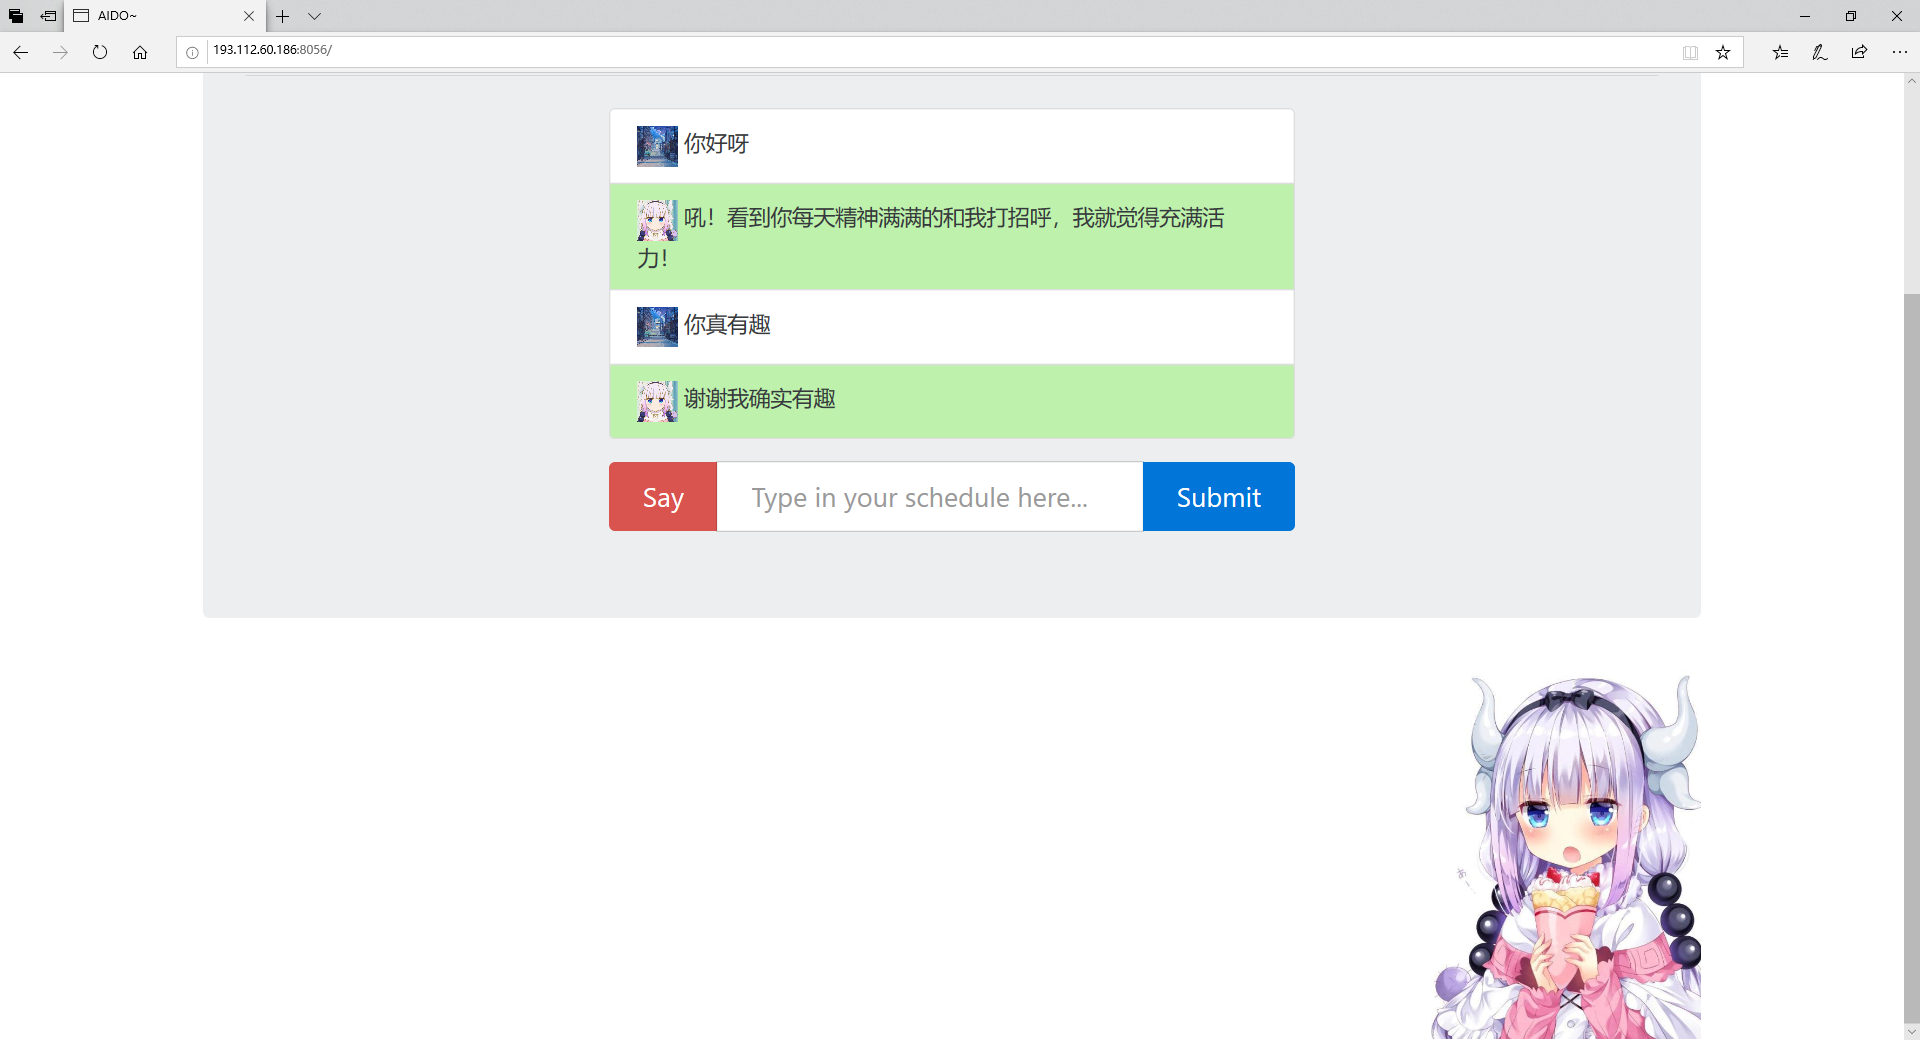
\includegraphics[width=15cm]{fig/chatting}
\end{figure}
\par 我们的机器人支持语言输入,按住say按钮就可以进行录音。录音文件就会保存到本地。同时,机器人也会根据语音进行相应的回答。用户可以通过与智能机器人交流,达到近似于与真人进行交流的体验。于此同时,下面的一系列功能都支持语音输入。
\item \textbf{日常查询功能:}AIDO可以根据用户输入的信息,解释相关概念。
\begin{figure}[H]
\centering
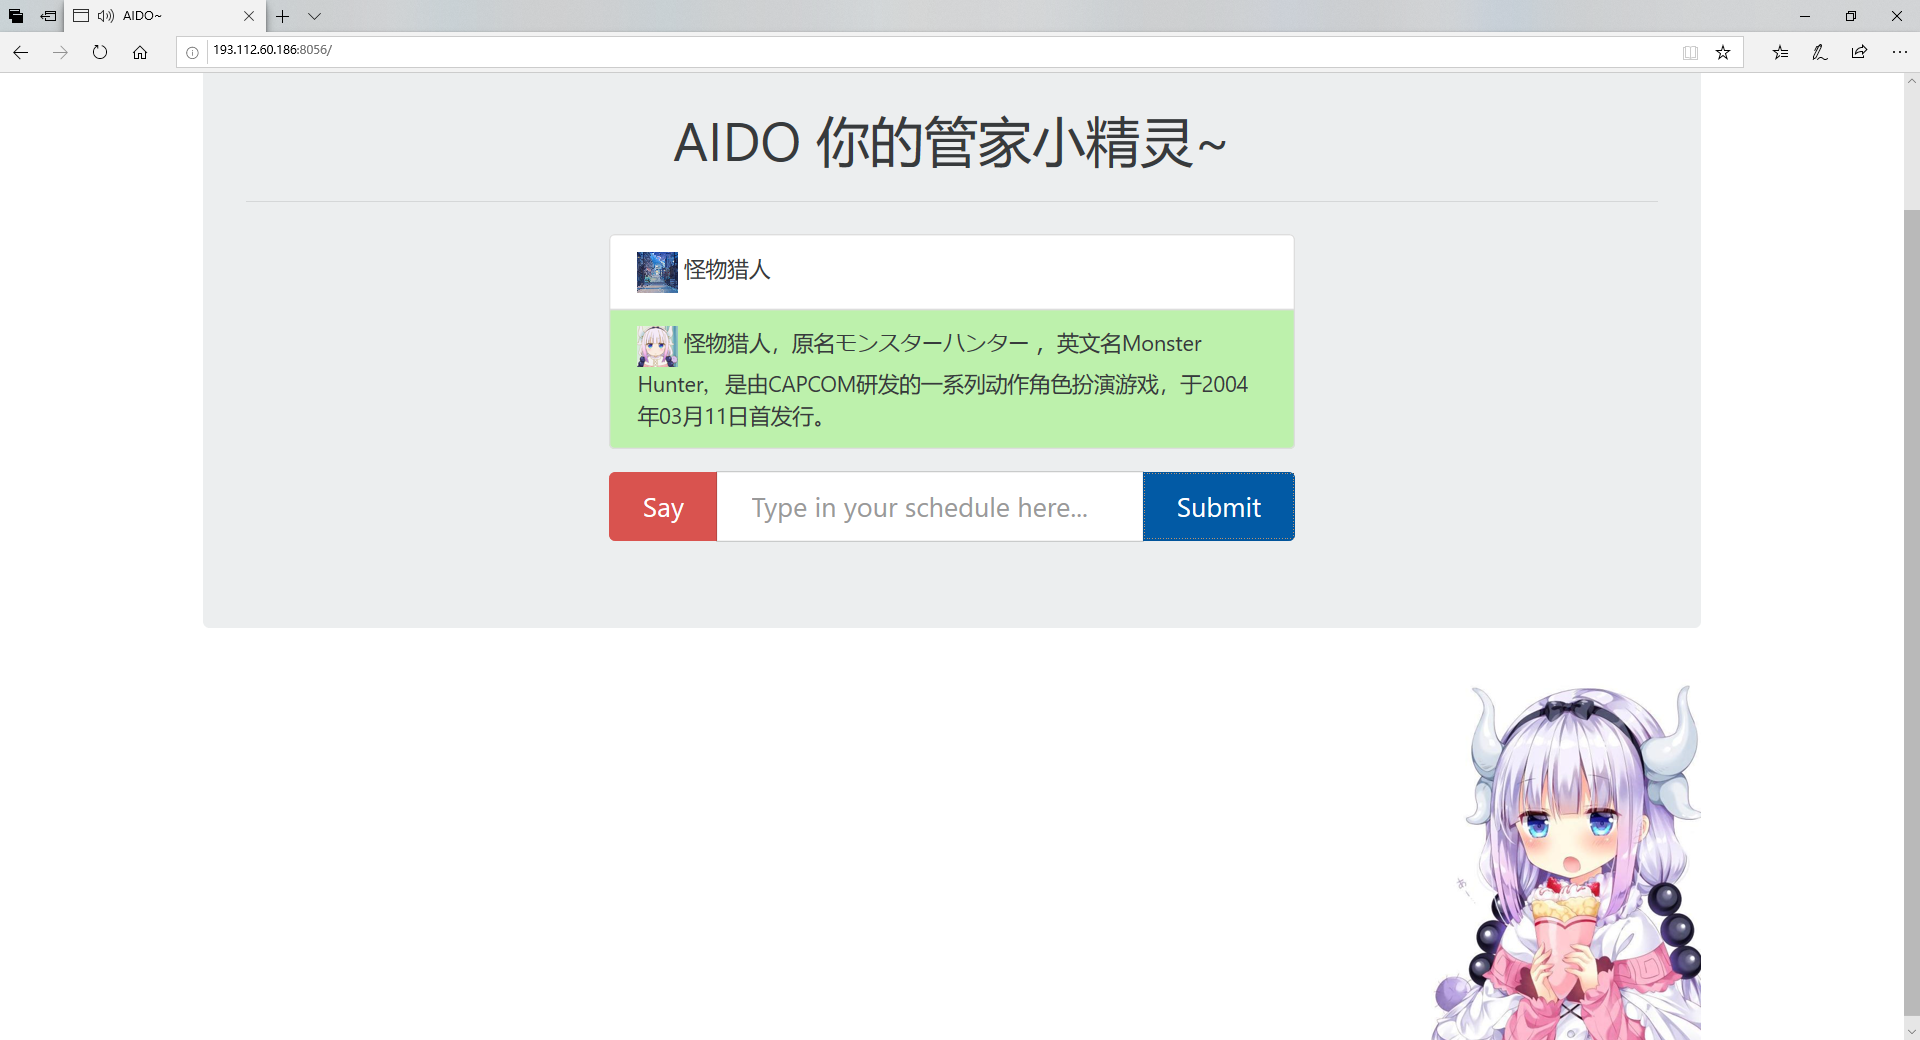
\includegraphics[width=15cm]{fig/wiki}
\end{figure}
\par 用户可以输入想要了解的人物/事务,机器人就会为用户提供对应概念的解释,此处机器人提供的解释主要来源于百度百科。
\item \textbf{添加任务功能:}AIDO可以实现帮用户添加任务事项的功能。
\begin{figure}[H]
\centering
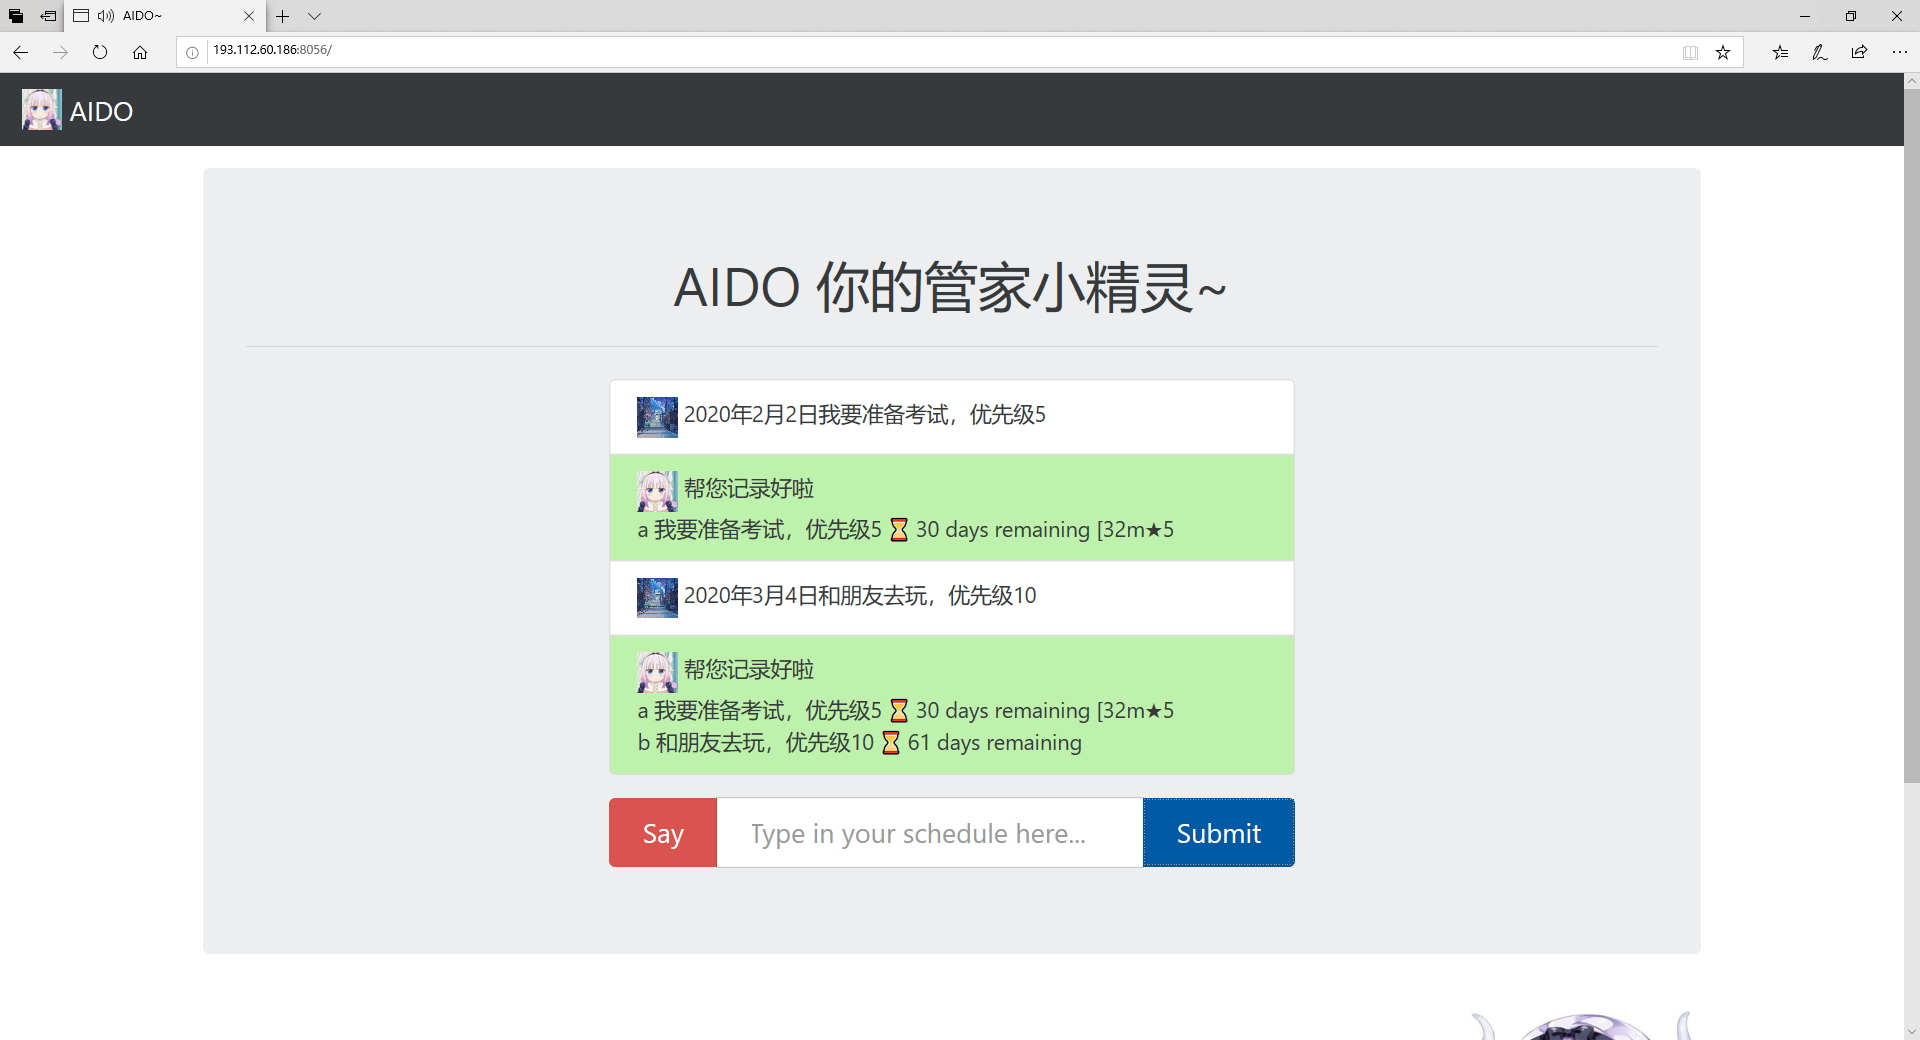
\includegraphics[width=15cm]{fig/add_task}
\end{figure}
\par 用户输入日期(****年*月*日)+任务,机器人将帮用户录入todolist,并自动计算距离deadline的时间。此外,支持给任务添加优先级。在任务中添加“优先级”+数字,奇迹人将自动检测任务的优先级并将高优先级的任务排在前面。
\item \textbf{删除任务功能:}AIDO可以实现帮助用户删除任务事项的功能。
\begin{figure}[H]
\centering
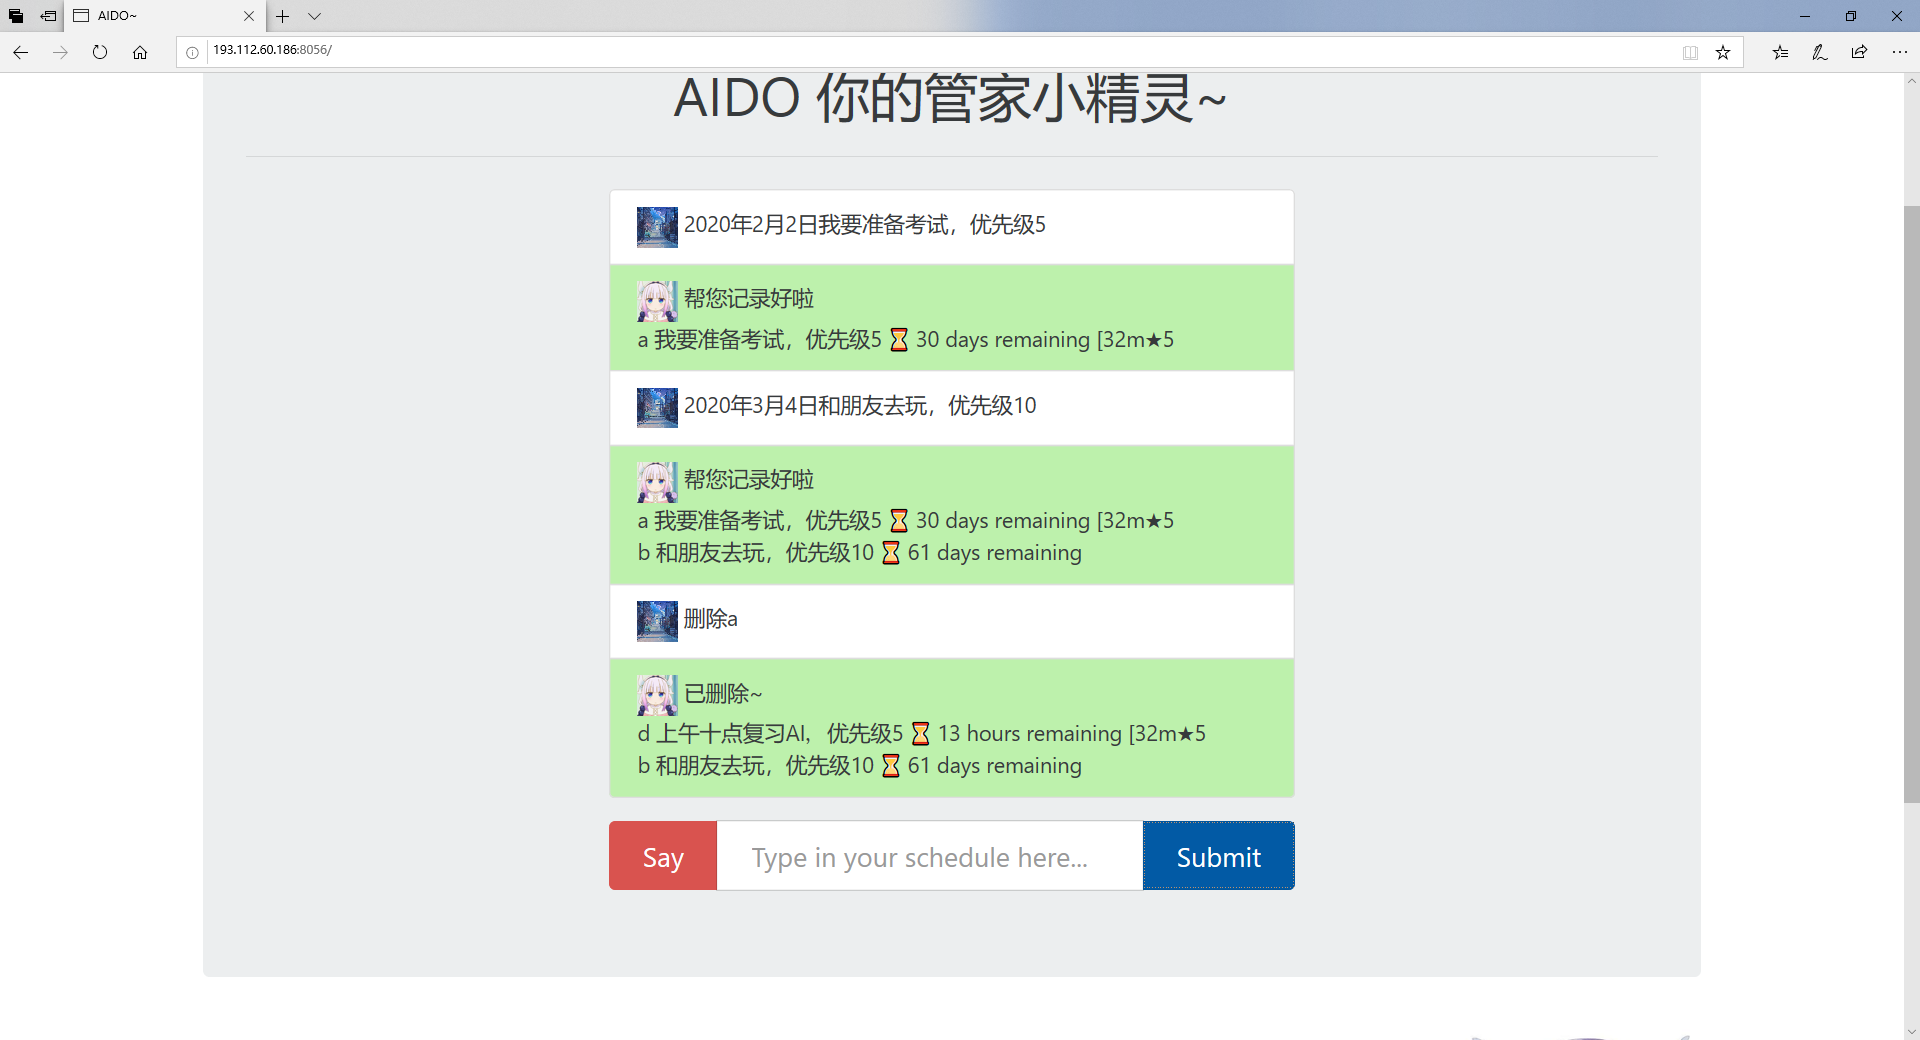
\includegraphics[width=15cm]{fig/del_task}
\end{figure}
\par 通过输入“删除”+任务对应的字母/数字,机器人就可以帮助用户删除对应的任务。
\item \textbf{查看待办事项功能:}AIDO允许用户查询当前剩余的待办事项。
\begin{figure}[H]
\centering
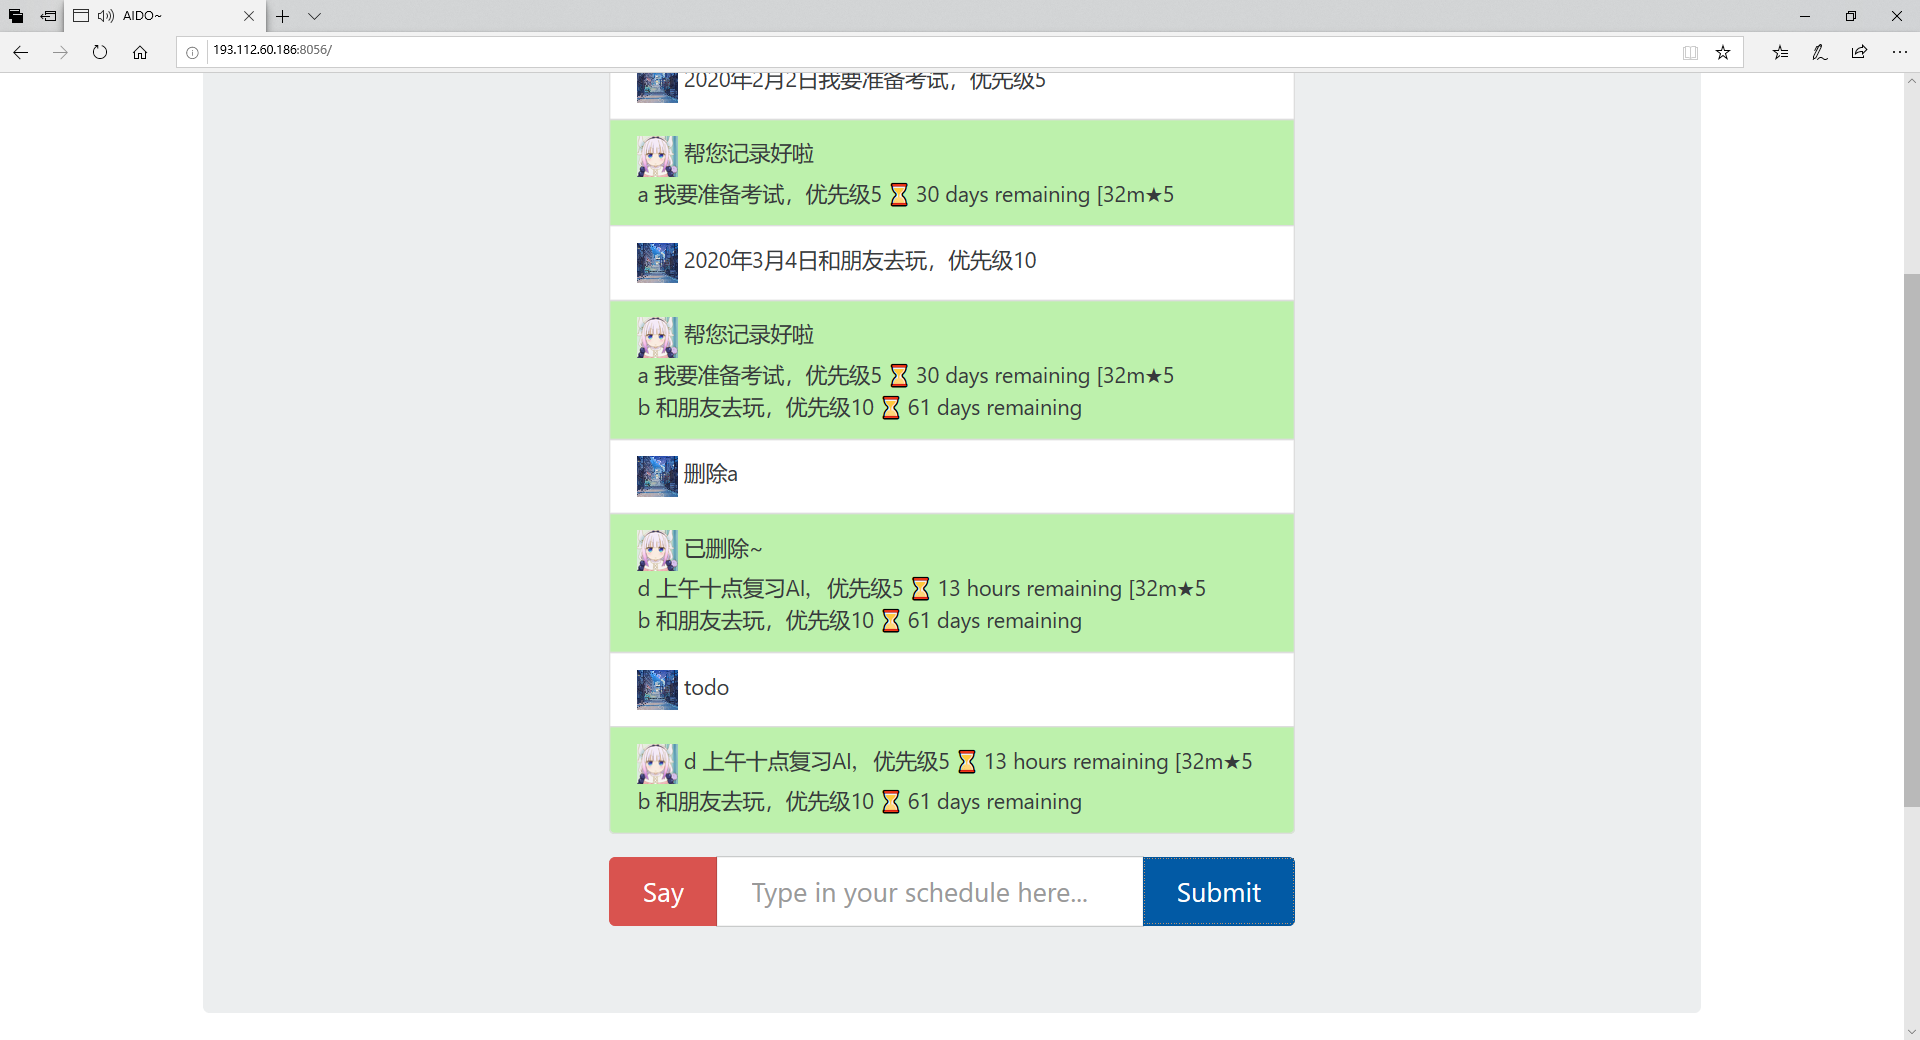
\includegraphics[width=15cm]{fig/ask_task}
\end{figure}
\par 通过输入“todo”,用户可以查看现有的所有待办事项的详细信息。
\end{itemize}
\par 我们的项目主要包含了以上功能,可以说,AIDO包含了todolist的核心功能,但同时加入了智能机器人这一辅助工具,使个人事务的管理可以统一使用语音输入这一手段进行管理,增加了效率和方便性,又使得应用场景更丰富,机器人可以协助解决除事务管理外的其它问题。同时,AIDO也提供了更为美观、友好的交互界面,给用户带来更好的体验。

\section{ER图与关系模式设计}
\subsection{ER图}
\par 本项目设计的ER图如下所示:
\begin{figure}[H]
\centering
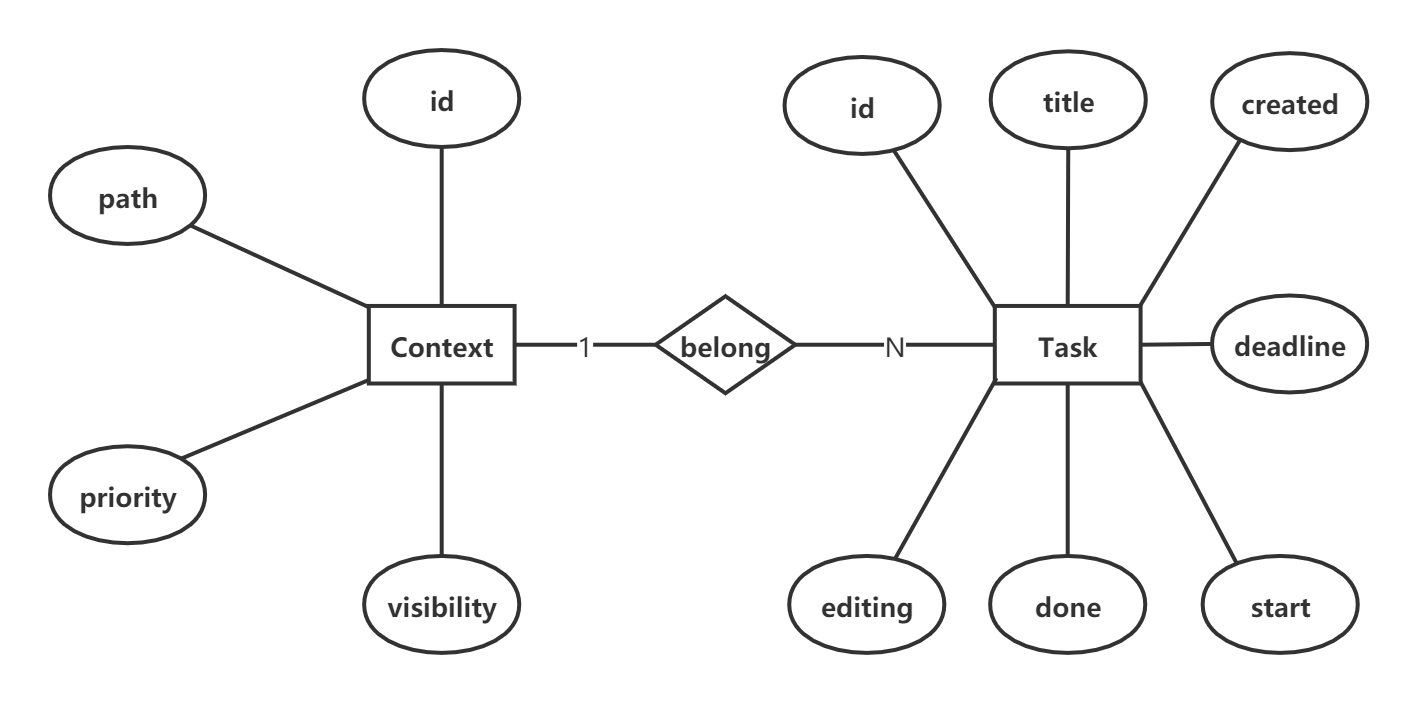
\includegraphics[width=15cm]{fig/er_design}
\end{figure}
\subsection{关系模式与建表语句}
\par 根据以上ER图,我们可以建立以下关系模式:
\begin{itemize}
\item \textbf{Task(\uline{id}, title, created, deadline, start, priority, done, \uwave{context}, content, editing)}
\begin{lstlisting}[language=SQL]
CREATE TABLE `Task` (
	`id`	INTEGER NOT NULL PRIMARY KEY AUTOINCREMENT UNIQUE,
	`title`	TEXT NOT NULL,
	`created`	TEXT NOT NULL DEFAULT (datetime('now')),
	`deadline`	TEXT,
	`start`	TEXT NOT NULL DEFAULT (datetime('now')),
	`priority`	INTEGER NOT NULL DEFAULT 1,
	`done`	TEXT,
	`context`	INTEGER NOT NULL REFERENCES Context(id) ON DELETE CASCADE
);
CREATE INDEX `DoneIndex` ON `Task` (`done`);
CREATE INDEX `DateCreatedIndex` ON `Task` (`created`);
ALTER TABLE Task ADD COLUMN `content` TEXT;
ALTER TABLE Task ADD COLUMN `editing` INTEGER NOT NULL DEFAULT 0;
\end{lstlisting}
\item \textbf{Context(\uline{id}, path, priority, visibility)}
\begin{lstlisting}[language=SQL]
CREATE TABLE `Context` (
	`id`	INTEGER NOT NULL PRIMARY KEY AUTOINCREMENT UNIQUE,
	`path`	TEXT NOT NULL UNIQUE,
	`priority`	INTEGER NOT NULL DEFAULT 1,
	`visibility`	TEXT NOT NULL DEFAULT 'normal'
);
INSERT INTO `Context` (path) VALUES ('');
CREATE INDEX `PathIndex` ON `Context` (`path` ASC);
\end{lstlisting}
\end{itemize}

\section{设计细节}
\par 本节主要介绍各个部分的设计细节,包括其中涉及的代码细节与SQL语句。

\subsection{todolist}
todolist的实现主要包含了四个模块,添加任务,删除任务, 修改任务以及查询任务。
\subsubsection{添加任务}
\par todolist中有任务的添加,以及环境(context)的添加。
\begin{itemize}
\item 任务添加
\begin{lstlisting}[language=SQL]
INSERT INTO Task (title, content, context {})
VALUES (?, ?, ? {})
\end{lstlisting}
\item 环境添加
\begin{lstlisting}[language=SQL]
INSERT INTO Context (path)
VALUES (?)
\end{lstlisting}
\item 将一个路径中的任务复制到另一路径
\begin{lstlisting}[language=SQL]
UPDATE Task
SET context = ?
WHERE context = (
	SELECT id FROM Context
	WHERE path = ?
)
\end{lstlisting}
\end{itemize}

\subsubsection{删除任务}
\par todolist中有对数据的删除操作,其中包括了删除任务,删除环境,以及删除满足某些要求的任务。
\begin{itemize}
\item 删除特定id的任务
\begin{lstlisting}[language=SQL]
DELETE FROM Task
WHERE id = ?
\end{lstlisting}
\item 删除特定路径的环境
\begin{lstlisting}[language=SQL]
DELETE FROM Context
WHERE path LIKE ?
\end{lstlisting}
\item 删除某时刻前产生,并且已完成的任务
\begin{lstlisting}[language=SQL]
DELETE FROM Task
WHERE done IS NOT NULL
AND created < ?
\end{lstlisting}
\end{itemize}

\subsubsection{修改任务}
\par todolist中有对任务的修改操作,其中主要是修改任务内容,或是更改任务的标记内容(完成标记以及编辑标记)。
\begin{itemize}
\item 修改特定id的任务
\begin{lstlisting}[language=SQL]
UPDATE Task SET {}
WHERE id = ?
\end{lstlisting}
\item 标注特定id的任务状态为完成
\begin{lstlisting}[language=SQL]
UPDATE Task SET done = datetime('now')
WHERE id = ?
AND done IS NULL
\end{lstlisting}
\item 标记特定未处于编辑的任务为编辑状态
\begin{lstlisting}[language=SQL]
UPDATE Task
SET editing = 1
WHERE id = ?
  AND editing = 0
\end{lstlisting}
\item 释放某任务的编辑状态
\begin{lstlisting}[language=SQL]
UPDATE Task
SET editing = 0
WHERE id = ?
\end{lstlisting}
\end{itemize}

\subsubsection{查询任务}
\par todolist中有如下的各种查询操作。
\begin{itemize}
\item 查询特定id的任务
\begin{lstlisting}[language=SQL]
SELECT t.*, c.path as ctx_path
FROM Task t JOIN Context c
ON t.context = c.id
WHERE t.id = ?
\end{lstlisting}
\item 根据路径查询环境id
\begin{lstlisting}[language=SQL]
SELECT id FROM Context
WHERE path = ?
\end{lstlisting}
\item 查询特定路径的环境是否存在
\begin{lstlisting}[language=SQL]
SELECT 1 FROM Context
WHERE path = ?
\end{lstlisting}
\item 查询特定路径环境包含的任务数和子环境数
\begin{lstlisting}[language=SQL]
SELECT COUNT(t.id)
FROM Task t
JOIN Context c
ON t.context = c.id
WHERE t.done IS NULL
AND c.path = ?
UNION ALL
SELECT COUNT(id)
FROM Context
WHERE path LIKE ?
\end{lstlisting}
\item 查询特定路径下的所有任务(这些任务直接在该目录下,不在子目录):
\begin{lstlisting}[language=SQL]
SELECT t.*, c.path as ctx_path
FROM Task t JOIN Context c
ON t.context = c.id
WHERE c.path = ?
  AND t.done IS NULL
  AND (c.path = ? OR c.visibility = 'normal')
  AND (datetime('now')) >= datetime(t.start)
ORDER BY
  priority DESC,
  COALESCE(
      julianday(deadline),
      julianday('9999-12-31 23:59:59')
    ) - julianday('now') ASC,
  created ASC
\end{lstlisting}
\item 查询最大的任务id
\begin{lstlisting}[language=SQL]
SELECT MAX(id)
FROM Task
\end{lstlisting}
\item 查询特定路径下特定标题的任务
\begin{lstlisting}[language=SQL]
SELECT t.*, c.path as ctx_path
FROM Task t JOIN Context c
ON t.context = c.id
WHERE t.title LIKE ?
  AND c.path LIKE ?
\end{lstlisting}
\end{itemize}

\subsection{对话机器人} %待修改
\subsection{交互界面} %待修改
\section{技术难点} %待修改
\subsection{后端设计} %待修改
\subsection{前端设计} %待修改
\section{结语}
\par 本项目至此便已圆满结束,在这个项目中确实学习到了很多在课堂上学习不到的知识,也提升了项目开发能力。我们有几个简单的感想:
\begin{itemize}
\item 实际的项目开发比原想的要复杂的多。对比以往有明确要求的各种大作业,这次的大作业只是给了基本的要求,要做什么项目、要怎么实现、要达到什么程度等都得自行决定。因此,这次的作业,前期的准备规划阶段对比以往的作业也尤为重要,小组内需要商讨项目内容,需要调查市场竞品,还得考虑到实际的开发时间等,所有这些都商量好之后才能进入之后的开发阶段,进行代码的实现与测试。
\item 代码的复杂使实现的过程也存在困难。这次的作业要求我们实现包含前端界面和后端服务器的一个完整程序。后端包含的两个模块虽然都有比较成熟的模板,但是实际开发过程中,配置代码运行的环境,以及两部分代码的衔接,实现原有代码没有的功能等,耗费了队友的大量精力。前端界面的开发虽然在前半学期的todolist中有练习过,但在实际的开发中这并不足够,所以也是一边学习一边实现。同时,在接口的对接时,两位队友也进行了大量的沟通。这也让我们反省我们的开发流程是否还有优化的空间,可能在前期进行规划的时候需要对各种模块端口进行更为明确的规定。
\end{itemize}
\par 总之,我感谢我两位队友与我的组队!面对工作量如此巨大的Project,队友的努力,让这个项目有坚持下去并圆满完成的可能!
\par 以及,十分感谢助教检查我们的项目,提出宝贵的建议,并不厌其烦地读完这篇冗长的报告。
\end{document}